\documentclass[10pt]{beamer}
% \documentclass[handout,10pt]{beamer}
\usepackage{my_style}

%%%%%%%%%%%%%%%%%%%%%%%%%%%%%%%%%%%%%%%%%%%%%%%%%%%%%%%%%%%%%%%%%%%%%%%%

\title[Math/CS 375]{Lecture 08 - B}
\subtitle{\S 8.4 Sparsity and Iterative Methods}

\begin{document}
% -------------------------------------------------
\begin{frame}
  \titlepage
\end{frame}
% -------------------------------------------------
\begin{frame}{Goals}
We will answer these questions:\\[3mm]
\begin{itemize}
    \item Under what condition does Jacobi converge?
    \item How are Jacobi and GS coded in practice?
    \item What are sparse matrices?
    \item Why is sparsity important for iterative solvers?
\end{itemize}
\end{frame}

\begin{frame}{Jacobi and GS}

\begin{block}{Jacobi Iteration}
    
$$
x^{(k)} = x^{(k-1)} + D^{-1}r^{(k-1)},
$$
\end{block}

\begin{block}{Gauss-Seidel Iteration}
$$
x^{(k)} = x^{(k-1)} + (D+C_L)^{-1}r^{(k-1)}
$$
\end{block}


\begin{example}
We saw that Jacobi was working for this example:
\[
A=\begin{bmatrix}
\;2 & -1\\
-1 & \;2
\end{bmatrix},
\qquad
b=\begin{bmatrix}
1\\[2pt] 0
\end{bmatrix},
\qquad
x^{(0)}=\begin{bmatrix}
0\\[2pt] 0
\end{bmatrix}.
\]
\end{example}


\question{Does Jacobi and GS always work?}
\end{frame}

%%%%%%%%%%%%%%%%%%%%%%%%%%%%%%%%%%%%%%%%%%%
\sectionframe{Convergence}
%%%%%%%%%%%%%%%%%%%%%%%%%%%%%%%%%%%%%%%%%%%


\begin{frame}{Direct vs. Iterative}

\begin{block}{What are we trying to solve?}
$$Ax=b$$
\end{block}

\begin{itemize}
    \item \textbf{Direct Solver}:  Each step works toward the exact solution $x^*$
    \begin{itemize}
        \item Too expensive for large problems 
        $$
        \text{Cost} = \mO(n^3)
        $$
    \end{itemize}
    \vfill
    \item \textbf{Iterative Solver}: Each step improves the entire solution vector $x^{(k)}\to x^{(k+1)}$
        \begin{itemize}
            \item Must worry about \textbf{convergence}
             $$\lim_{k\to\infty} e^{(k)}=0$$
        \end{itemize}
    \vfill
    \keyidea{Convergence is always a concern for iterative methods.}
\end{itemize}
    
\end{frame}

%%%%%%%%%%%%%%%%%%%

\begin{frame}{Error vs. Residual}


    \begin{block}{Error Vector}
     The $k^{th}$ \textbf{error} vector is 
    $$
    e^{(k)} = x^*-x^{(k)}
    $$
    where $x^*$ is the exact solution to $Ax=b$
    \end{block}
    \vfill 

    \begin{block}{Residual Vector}
    The $k^{th}$ \textbf{residual} vector is 
        $$ r^{(k)} := b - Ax^{(k)}$$
    \end{block}
    \vfill

    \begin{block}{Their Relation}    
    They are related to each other
        \begin{align*}
        r^{(k)} &= b - Ax^{(k)}\\
        &= Ax^{*} - A x^{(k)}\\
        &=A e^{(k)}
        \end{align*}
    \end{block}


\end{frame}



%%%%%%%%%%%%%%%%%%%

% \begin{frame}{Error Analysis}{Part 1}
% \begin{itemize}
%     \item Jacobi and GS both have the form
% \begin{equation*}
% 	x^{(k)} = x^{(k-1)} + Q^{-1}r^{(k-1)}
% \end{equation*}
% \item By subtracting both sides from the \textbf{true solution} $x^{*}$
% \begin{equation*}
% 	x^*-x^{(k)} = x^*-x^{(k-1)} - Q^{-1}r^{(k-1)}
% \end{equation*}
% \item Substitute \textbf{error }$e^{(k)} = x^* - x^{(k)}$ and $r^{(k-1)} = Ae^{(k-1)}$:
% \begin{equation*}
% e^{(k)} = e^{(k-1)} - Q^{-1}Ae^{(k-1)}
% \end{equation*}
% and then factor out the vector $e^{(k-1)}$
% \begin{equation*}
% e^{(k)} = (I -  Q^{-1}A) e^{(k-1)}
% \end{equation*}
% \item By induction, we finally get our desired equation
% \begin{equation*}
% e^{(k)} = (I -  Q^{-1}A)^{k} e^{(0)}
% \end{equation*}
% \end{itemize}
% \end{frame}

%%%%%%%%%%%%%%%%%%%%%%%%%%%%%%%%%%%%%%%%%%%

\begin{frame}{Error Analysis}{Part 1}

\begin{itemize}
    \item Start with the iteration:
    \[
        x^{(k)}=x^{(k-1)}+Q^{-1}r^{(k-1)}.
    \]

    \item Subtract from the exact solution:
    \[
        x^*-x^{(k)}
        =x^*-x^{(k-1)}-Q^{-1}r^{(k-1)}.
    \]

    \item Substitute $e^{(k)}=x^*-x^{(k)}$
    and $r^{(k-1)}=Ae^{(k-1)}$:
    \[
        e^{(k)}
        =e^{(k-1)}-Q^{-1}Ae^{(k-1)}.
    \]
\end{itemize}

\onslide<2>{
\begin{block}{How the Error Changes}
\[
    e^{(k)}=Te^{(k-1)},
    \qquad
    T:=I-Q^{-1}A.
\]
\end{block}
}

\end{frame}

\begin{frame}{Error Analysis}{Part 2}

\begin{itemize}
    \item Apply the error relation repeatedly:
    \[
        e^{(k)}
        =Te^{(k-1)}
        =T^2e^{(k-2)}
        =\cdots=T^ke^{(0)}.
    \]

    \item Using a compatible vector norm and
    its induced matrix norm:
    \begin{align*}
        \|e^{(k)}\|
        &=\|T^ke^{(0)}\|\\
        &\le \|T^k\|\,\|e^{(0)}\|\\
        &\le \|T\|^k\,\|e^{(0)}\|.
    \end{align*}
\end{itemize}

\begin{block}{A Sufficient Condition for Convergence}
\[
    \|T\|<1
    \quad\Longrightarrow\quad
    \|e^{(k)}\|\longrightarrow0.
\]
\end{block}

\end{frame}

%%%%%%%%%%%%%%%%%%%%%%%%%%%%%%%%%%%%%%%%%%%
\begin{frame}{What Does the Bound Tell Us?}

\begin{block}{Error Bound}
\[
    \|e^{(k)}\|\le \|T\|^k\|e^{(0)}\|.
\]
\end{block}

\begin{itemize}
    \item If $\|T\|<1$, convergence is guaranteed.

    \bigskip

    \item If $\|T\|\ge1$, this bound is inconclusive.
\end{itemize}

\keyidea{
As long as $Q$ is chosen in a way that 
$$
\|I-Q^{-1}A \|<1
$$
stationary solvers will converge.
}

\end{frame}
%%%%%%%%%%%%%%%%%%%%%%%%%%%%%%%%%%%%%%%%%%%
\begin{frame}{More Results}

    \begin{block}{Divergence}
    A stationary iterative solver $x^{(k)} = x^{(k-1)} + Q^{-1}r^{(k-1)}$ will diverge if 
        $$\|I-Q^{-1}A\|>1$$
    \end{block}

    \begin{block}{Convergence Rate}
    Since error decreases like 
    $$
        \|e^{(k+1)}\| = \|I-Q^{-1}A\|\,\|e^{(k)}\|
    $$
    the quantity $\|I-Q^{-1}A\|$ acts as the convergence rate.
    \end{block}

    \vspace{3mm}
    The smaller this number is $\|I-Q^{-1}A\|$, the faster the iteration converges.
    
\end{frame}
%%%%%%%%%%%%%%%%%%%%%%%%%%%%%%%%%%%%%%%%%%%
\begin{frame}{Convergence Rate}
\begin{itemize}
    \item The quantity $$r(Q)=\|I-Q^{-1}A\|$$ 
    depending on $Q$ controls how quickly the iterative method converges\\[3mm]

    \item Choices for $Q$
    \begin{itemize}
        \item Jacobi $Q=D$
        \item GS $Q=D+C_L$  
        \item There are several more but we focus only on these two
    \end{itemize}

    \question{\begin{itemize}
        \item How many FLOPs do each method cost per iteration? 
        \item Which method has a lower value of $r(Q)$? 
        \item Which method has a lower runtime? 
        \item Does the size of the matrix matter for convergence rate?
    \end{itemize}}
\end{itemize}
\end{frame}
%%%%%%%%%%%%%%%%%%%%%%%%%%%%%%%%%%%%%%%%%%%
\begin{frame}{Convergence Example}
\begin{example}
    Will Jacobi iteration for the matrix 
        $$A = \begin{bmatrix}
    3 &-1 & 0\\
    -1 &3 &-1\\
    0 &-1 &2
    \end{bmatrix}$$
    converge or diverge?
\end{example}
    
\begin{itemize}
    \item We know that for Jacobi iteration
    $$
    Q = \begin{bmatrix}
    3 &0 & 0\\
    0 &3 &0\\
    0 &0 &2
    \end{bmatrix} \quad Q^{-1} = \begin{bmatrix}
    1/3 &0 & 0\\
    0 & 1/3 &0\\
    0 &0 &1/2
    \end{bmatrix}
    $$
\item We have 
    $$ I - Q^{-1}A = \begin{bmatrix}
    1 &0 & 0\\
    0 &1 &0\\
    0 &0 &1
    \end{bmatrix} - 
    \begin{bmatrix}
    1 &-1/3 & 0\\
    -1/3 &1 &-1/3\\
    0 &-1/2 &1
    \end{bmatrix}=
    \begin{bmatrix}
    0 & 1/3 & 0\\
    1/3 &0 & 1/3\\
    0 & 1/2 &0
    \end{bmatrix}
    $$
\item $\| I - Q^{-1}A\|_\infty = 2/3 < 1 \implies $ convergent
\end{itemize}
\end{frame}
%%%%%%%%%%%%%%%%%%%%%%%%%%%%%%%%%%%%%%%%%%%
\begin{frame}{Diagonally Dominant}
\define{Definition: Diagonal Dominance}{
    An $n\times n$ matrix $A$ is \textbf{strictly diagonally dominant} if
    \begin{equation*}
    	|a_{ii}| > \sum_{j=1,j\ne i}^{n} |a_{ij}|
    \end{equation*}
    for all $i$. 
}

    Example: 
        $$A = \begin{bmatrix}
    3 &-1 & 0\\
    -1 &3 &-1\\
    0 &-1 &2
    \end{bmatrix}$$
\begin{itemize}
    \item Row 1: $|3| > |-1| + |0| = 1 $ 
    \item Row 2: $|3| > |-1| + |-1| = 2 $
    \item Row 3: $|2| > |0| + |-1| = 1$
    \item Therefore, $A$ is diagonally dominant 
\end{itemize}
\end{frame}
%%%%%%%%%%%%%%%%%%%%%%%%%%%%%%%%%%%%%%%%%%%
\begin{frame}{Sufficient Convergence Criterion}
\begin{theorem}
	If $A$ is strictly diagonally dominant, then the Jacobi and Gauss-Seidel methods converge for any initial guess $x^{(0)}$.
\end{theorem}


\keyidea{
 Checking the convergence criterion
        $$\|I-Q^{-1}A\|<1$$
can be a hassle. Checking for diagonal dominance is much faster and will guarantee convergence.
}
\end{frame}

\begin{frame}{Why Diagonal Dominance Works}{Jacobi}

\begin{itemize}
    \item For Jacobi, since $T=I-D^{-1}A$, the diagonal elements are always zero
    \[
        t_{ii}=0,
    \]

    \item The infinity norm is therefore the largest sum of the remaining values
    \[
            t_{ij}=-\frac{a_{ij}}{a_{ii}}
        \quad (i\ne j),\qquad
        \|T\|_\infty
        =
        \max_i
        \frac{\sum_{j\ne i}|a_{ij}|}{|a_{ii}|}.
    \]
\end{itemize}

\begin{block}{Strict Diagonal Dominance}
\[
    |a_{ii}|>\sum_{j\ne i}|a_{ij}|
    \quad\Longrightarrow\quad 
    \frac{\sum_{j\ne i}|a_{ij}|}{|a_{ii}|}<1
    \quad\Longrightarrow
    \|T\|_\infty<1.
\]
\end{block}


\end{frame}

%%%%%%%%%%%%%%%%%%%%%%%%%%%%%%%%%%%%%%%%%%%
\sectionframe{Component-Wise Implementation}
%%%%%%%%%%%%%%%%%%%%%%%%%%%%%%%%%%%%%%%%%%%

\begin{frame}{Recall: Why do we need iterative solvers?}

\begin{center}
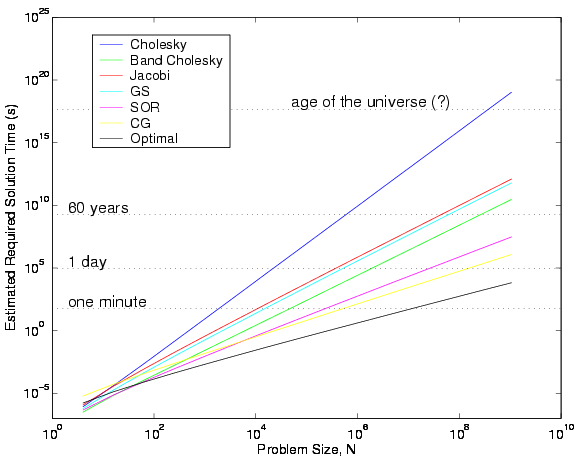
\includegraphics[scale=0.42]{figs/solvers.png}
\end{center}

\keyidea{For problems of size $N=10^6$ and greater, direct solvers are not feasible. }

\end{frame}

%%%%%%%%%%%%%%%%%%%%%%%%%%%%%%%%%%%%%%%%%%%
\begin{frame}{What Must We Compute?}

\begin{itemize}
    \item Every stationary iteration needs a correction:
\end{itemize}

\begin{block}{Solve and Update}
\[
    Qc^{(k)}=r^{(k)},
    \qquad
    x^{(k+1)}=x^{(k)}+c^{(k)}.
\]
\end{block}

\begin{itemize}
    \item Jacobi: $Q=D$.
    \item Gauss-Seidel: $Q=D+C_L$.
\end{itemize}
    \vfill 
\begin{block}{Why it matters:}
    All vectors and matrices created in Matlab requires RAM.
\end{block}



\end{frame}

\begin{frame}[fragile]{Explicitly Constructing $Q$}

\begin{lstlisting}
% A is loaded
Q = diag(diag(A));   % Jacobi: build diagonal matrix
x = x0;
for k = 1:kmax
    r = b - A*x;
    if norm(r) <= tol
        break
    end
    c = Q\r;
    x = x + c;
end
\end{lstlisting}

\begin{block}{Memory Requirement}
\begin{itemize}
    \item Matrix $A$
    \item Matrix $Q$
    \item Vectors $x$, $r$, and $c$
\end{itemize}
\end{block}
\end{frame}

%%%%%%%%%%%%%%%%%%%%%%%%%%%%%%%%%%%%%%%%%%%

\begin{frame}[fragile]{Checking Memory}
\begin{itemize}

    \item Use the command \texttt{whos} to see how much memory a variable costs

    \begin{lstlisting}
>> A = zeros(10000,10000);

>> whos A
  Name          Size                   Bytes  Class     Attributes
  A         10000x10000            800000000  double           
\end{lstlisting}
    \vfill
    \item A $10,000\times10,000$ matrix takes up 800 Megabytes of RAM
    \vfill
    \item Even the zeros take up memory 
    \vfill 
    \onslide<2>{
    \question{
    What if $A$ is $1,000,000$ by $1,000,000$?
    }
    }
\end{itemize}
\end{frame}
%%%%%%%%%%%%%%%%%%%%%%%%%%%%%%%%%%%%%%%%%
%%%%%%%%%%%%%%%%%%%%%%%%%%%%%%%%%%%%%%%%%%%
\begin{frame}{The Storage Problem}

\begin{itemize}
    \item Suppose $A$ is $10^6\times10^6$.
    \vfill 
    \item Each number in $A$ is stored in FP64 $\implies$ each number is 8 bytes
    \vfill 
    \item Any variable created in Matlab takes up Dynamic Random Access Memomory (DRAM)
    \vfill 
    \item Storing another dense double-precision matrix $Q$
    requires:
\end{itemize}

\begin{block}{Additional Memory}
\[
    8(10^6)^2 \text{ bytes}
    =8\times10^{12}\text{ bytes}
    =\boxed{8\text{ TB of RAM}}. 
\]
\end{block}

\keyidea{We need a way to an alternative way to program iterative solvers due to memory limitations.}

\end{frame}


%%%%%%%%%%%%%%%%%%%%%%%%%%%%%%%%%%%%%%%%%%%
\begin{frame}[fragile]{Coding the Matrix as a Loop}

\begin{block}{Issue}
    Don't have enough memory to construct $Q$.
\end{block}
\begin{block}{Solution}
    Code the action of $Q^{-1}$ rather than the actual matrix.
\end{block}

\begin{itemize}
    \item Instead of $D^{-1}b$ like this:
\begin{lstlisting}
D\b
\end{lstlisting}   
    \item We can code the action of $D^{-1}b$ in a loop
\begin{lstlisting}
for i = 1:n
    b(i)/A(i,i)
end
\end{lstlisting}
      
\end{itemize}
\end{frame}

%%%%%%%%%%%

\begin{frame}{Use the Entries of $A$ Directly}

\begin{block}{General Update}
\[
    Qc^{(k)}=r^{(k)},
    \qquad
    x^{(k+1)}=x^{(k)}+c^{(k)}.
\]
\end{block}

\begin{block}{Jacobi: Independent Divisions}
\[
    c_i=\frac{r_i}{a_{ii}}.
\]
\end{block}

\begin{block}{Gauss-Seidel: Forward Substitution}
\[
    c_i=
    \frac{r_i-\displaystyle\sum_{j=1}^{i-1}a_{ij}c_j}
         {a_{ii}},
    \qquad i=1,\ldots,n.
\]
\end{block}

\keyidea{
We can solve $Qc=r$ without storing $Q$ separately.
}

\end{frame}



%%%%%%%%%%%%%%%%%%%%%%%%%%%%%%%%%%%%%%%%%%%
\begin{frame}[fragile]{Jacobi: Vector vs. Component-Wise Form}

    \begin{block}{Vector-update Form}
        \begin{equation*}
        x^{(k+1)} = -D^{-1}((C_L + C_U)x^{(k)}+b)
        \end{equation*}
    \end{block}
    \begin{block}{Component-Wise Form}
    For $i= 1,2,\ldots, n$
        \begin{equation*}
        x_{i}^{(k+1)} = -\sum_{j=1,j\ne i}^{n} \left(\frac{a_{ij}}{a_{ii}}\right) x_{j}^{(k)} + \frac{b_{i}}{a_{ii}}
        \end{equation*} 
    \end{block}

    \vspace{3mm}
    \begin{itemize}
        \item Both are equivalent forms of Jacobi iteration
        \item Component-wise form does not require $D$, $C_U$, $C_L$
        \item The component-wise form is meant to be written a loop
    \end{itemize}


\end{frame}

%%%%%%%%%%%%%%%%%%%%%%%%%%%%%%%%%%%%%%%%%%%

\begin{frame}{Component-Wise Gauss-Seidel}
\begin{itemize}

    \begin{block}{Vector-update Form}
        \begin{equation*}
        x^{(k)} = -(D+C_L)^{-1}C_U x^{(k-1)} + (D+C_L)^{-1}b
        \end{equation*}
    \end{block}
    \begin{block}{Component-wise Form}
    For $i= 1,2,\ldots, n$
        \begin{equation*}
        x_{i}^{(k)} = -\sum_{j=1}^{i-1} \left(\frac{a_{ij}}{a_{ii}}\right) x_{j}^{(k)} -\sum_{j=i+1}^{n} \left(\frac{a_{ij}}{a_{ii}}\right) x_{j}^{(k-1)} + \frac{b_{i}}{a_{ii}}
        \end{equation*} 

    \end{block}
\vspace{5mm}

\item GS also has a component-wise form 

\end{itemize}
\end{frame}



%%%%%%%%%%%%%%%%%%%%%%%%%%%%%%%%%%%%%%%%%%%%
\sectionframe{Sparsity}
%%%%%%%%%%%%%%%%%%%%%%%%%%%%%%%%%%%%%%%%%%%%

\begin{frame}{Sparse Matrices}

\define{Sparse Matrix}{
\begin{itemize}
    \item A matrix is \textbf{sparse} if most of its entries are zero.
    \item Let $A$ be $n\times n$. We assume each row has $m\ll n$ nonzeros.
\end{itemize}
}

\begin{itemize}
    \item Many useful applications
    \begin{itemize}
        \item Differential equations.
        \item Circuits and networks.
        \item Structural engineering.
    \end{itemize}

 \item Example: Tridiagonal Toeplitz Matrix
\end{itemize}
\[
A=
\begin{bmatrix}
4  & -1 &    &        &   \\
-1 & 4  & -1 &        &   \\
   & -1 & 4  & \ddots &   \\
   &    & \ddots & \ddots & -1\\
   &    &        & -1 & 4
\end{bmatrix}
\]

\end{frame}

%%%%%%%%%%%%%%%%%%%%%%%%%%%%%%%%%%%%%%%%%%%%

\begin{frame}{Example: A Tridiagonal Matrix}

\[
A=
\begin{bmatrix}
4  & -1 &    &        &   \\
-1 & 4  & -1 &        &   \\
   & -1 & 4  & \ddots &   \\
   &    & \ddots & \ddots & -1\\
   &    &        & -1 & 4
\end{bmatrix}
\]

\begin{itemize}
    \item Blank entries are zero.
    \item At most $m=3$ nonzeros per row.
    \item Only $3n-2$ nonzeros out of $n^2$ entries.
\end{itemize}

\question{
Why store all those zeros?
}

\end{frame}

%%%%%%%%%%%%%%%%%%%%%%%%%%%%%%%%%%%%%%%%%%%%

\begin{frame}{Sparse Storage}

\begin{block}{Dense Storage}
Store all $n^2$ entries, including zeros.
\[
    \text{Memory}=\mO(n^2).
\]
\end{block}

\begin{block}{Sparse Storage}
Store nonzero values and indexing information.
\[
    \text{Memory}=\mO(mn),
\]
where $m$ is the maximum number of nonzeros per row.
\end{block}

\keyidea{
If $m$ stays fixed as $n$ grows, storage grows linearly.
}

\end{frame}



%%%%%%%%%%%%%%%%%%%%%%%%%%%%%%%%%%%%%%%%%%%%%%%%%%%%%%%%%%

\begin{frame}[fragile]{Matlab Commands}
\begin{itemize}
    \item \texttt{gallery()} - construct various types of matrices 
    \begin{itemize}
        \item \texttt{doc gallery} for details
    \end{itemize}
    \item \texttt{numel(A)} - number of elements in $A$
    \item \texttt{nnz(A)} - number of non-zero elements in $A$
    \item \texttt{sparse(A)} - create a sparse version of $A$
    \item \texttt{full(A)} - create a dense version of $A$
    \item \text{whos A} - view memory size of $A$

\end{itemize}
\begin{lstlisting}
>> A = gallery('clement',5)  % dense 5x5 Clement matrix 
A =
     0     1     0     0     0
     4     0     2     0     0
     0     3     0     3     0
     0     0     2     0     4
     0     0     0     1     0

>> fprintf('Sparsity ratio: %.2f\n',nnz(A)/numel(A))
Sparsity ratio: 0.32
\end{lstlisting}
\end{frame}

\begin{frame}[fragile]{Sparse vs. Full}
\begin{lstlisting}
>> A = gallery('clement',5);
>> whos A
  Name      Size            Bytes  Class     Attributes
  A         5x5               200  double     

>> A = sparse(A)
A =
   (2,1)        4
   (1,2)        1
   (3,2)        3
   (2,3)        2
   (4,3)        2
   (3,4)        3
   (5,4)        1
   (4,5)        4

>> whos A
  Name      Size            Bytes  Class     Attributes
  A         5x5               176  double    sparse    
\end{lstlisting}

\end{frame}
%%%%%%%%%%%%%%%%%%%%%%%%%%%%%%%%%%%%%%%%%%
\begin{frame}[fragile]{Storage Format}
\begin{lstlisting}
>> A = sparse(A)
A =
   (2,1)        4
   (1,2)        1
   (3,2)        3
   (2,3)        2
   (4,3)        2
   (3,4)        3
   (5,4)        1
   (4,5)        4  
\end{lstlisting}
\begin{itemize}
    \item A \texttt{sparse} matrix in Matlab is stored as a pair between index and value
    \item For example, the first line \texttt{(2,1)}  \texttt{4} means $A_{21}=4$
\end{itemize}
\keyidea{Zeroes do not take up memory!}
\end{frame}


%%%%%%%%%%%%%%%%%%%%%%%%%%%%%%%%%%%%%%%%%%%%

\begin{frame}{Fill-in}

\begin{itemize}

    \item Elimination-based solvers can create new nonzeros.
\end{itemize}

$$
A \text{ is sparse} \nRightarrow L,U \text{ are sparse}
$$


\define{Fill-in}{
If a direct solver creates non-zero elements in the factorization where there were originally zero elements, it is called \textbf{fill-in}.
}

\begin{itemize}
    \item Fill-in increases memory cost. 
    \item Reordering may reduce fill-in.
\end{itemize}

\keyidea{
Direct solvers are not the most suited for handling sparse $A$ matrices.
}


\end{frame}

%%%%%%%%%%%%%%%%%%%%%%%%%%%%%%%%%%%%%%%%%%%%%%%%%%%%%%%%%%
\begin{frame}{Fill-in Example}
\begin{itemize}
    \item Consider what happens if you attempt LU factorization on the matrix 
    $$
    A = \begin{bmatrix} 
    4 & -1 & \cdots & -1 \\
    4 & 4 &  &\\
    \vdots & & \ddots &  \\
    4 & &  & 4
    \end{bmatrix}
    $$
     \item This matrix has exactly $3n-2$ non-zero elements out of $n^2$

     \item But after one step of GE 
     $$
    \begin{bmatrix} 
    4 & -1 & \cdots & -1 \\
    4 & 4 &  &\\
    \vdots & & \ddots &  \\
    4 & &  & 4
    \end{bmatrix} \longrightarrow
    \begin{bmatrix} 
    4 & -1& -1& \cdots & -1 \\
    0 & 5 & 1 &\cdots&1\\
    0 & 1 & 5 &\cdots&1\\
    \vdots &\vdots & & \ddots &\vdots  \\
    0 &1 & 1  & \cdots& 5
    \end{bmatrix}
     $$
     \item This is \textbf{fill-in}
\end{itemize}
\end{frame}


%%%%%%%%%%%%%%%%%%%%%%%%%%%%%%%%%%%%%%%%%%
\sectionframe{Sparsity for Iterative Solvers}
%%%%%%%%%%%%%%%%%%%%%%%%%%%%%%%%%%%%%%%%%%

\begin{frame}[fragile]{Make $A$ and $Q$ Sparse}

\begin{lstlisting}
% A is loaded as a sparse matrix
n = size(A,1);
Q = spdiags(diag(A), 0, n, n); % for Jacobi
% Q = tril(A);                 % for GS
x = x0;
for k = 1:kmax
    r = b - A*x;
    if norm(r) <= tol
        break
    end
    c = Q\r;
    x = x + c;
end
\end{lstlisting}

\begin{itemize}
    \item For iterative solvers, let $Q$ be sparse
    \item You can operate with \texttt{Q} as if it's a regular matrix
\end{itemize}

\question{What is the bottleneck here?}

\end{frame}

%%%%%%%%%%%%%%%%%%%%%%%%%%%%%%%%%%%%%%%%%%

\begin{frame}{Sparse Matrix-Vector Multiplication}

\begin{itemize}
    \item Each row computes a dot product:
    \[
        (Ax)_i=\sum_{j=1}^{n}a_{ij}x_j.
    \]

    \item Sparse operations skip the zero entries:
    \[
        (Ax)_i=\sum_{j:\,a_{ij}\ne0}a_{ij}x_j.
    \]
\end{itemize}

\begin{block}{At Most $m$ Nonzeros per Row}
\[
    \underbrace{n}_{\text{rows}}
    \times
    \underbrace{\mO(m)}_{\text{work per row}}
    =\mO(mn).
\]
\end{block}

\keyidea{
Calculating $r=b-Ax$ normally costs $\mO(n^2)$ but only $\mO(nm)$ if it's sparse.
}

\end{frame}

%%%%%%%%%%%%%%%%%%%%%%%%%%%%%%%%%%%%%%%%%%

% \begin{frame}[shrink]{Cost per Iteration}{Think $m=5$, $n=1000$}
    
%     \begin{block}{One Jacobi Iteration}
%         \begin{equation*}
%         x_{i}^{(k)} = -\sum_{j=1,j\ne i}^{n} \left(\frac{a_{ij}}{a_{ii}}\right) x_{j}^{(k-1)} + \frac{b_{i}}{a_{ii}}, \quad (i = 1 : n)
%         \end{equation*} 
%     \begin{itemize}
%         \item \textit{If $A$ is sparse}, this is $\mO(mn)$

%     \end{itemize}
%     \end{block}

%     \begin{block}{One GS Iteration}
%         \begin{equation*}
%         x_{i}^{(k)} = -\sum_{j=1}^{i-1} \left(\frac{a_{ij}}{a_{ii}}\right) x_{j}^{(k)} -\sum_{j=i+1}^{n} \left(\frac{a_{ij}}{a_{ii}}\right) x_{j}^{(k-1)} + \frac{b_{i}}{a_{ii}} \quad (i = 1 : n)
%         \end{equation*} 
%     \begin{itemize}
%     \item Normally would be $\mO(n^2)$
%     \item If $A$ is sparse, $\mathcal{O}(mn)$ 

%     \end{itemize}
%     \end{block}
% \end{frame}

%%%%%%%%%%%%%%%%%%%%%%%%%%%%%%%%%%%%%%%%%%

\begin{frame}{Cost per Iteration}

\begin{itemize}
    \item Assume at most $m$ nonzeros per row.
\end{itemize}

\begin{block}{Both Methods: Compute the Residual}
\[
    r=b-Ax
    \qquad \text{cost: }\mO(mn).
\]
\end{block}

\begin{block}{Compute the Correction}
\[
\begin{array}{lll}
    \text{Jacobi:} & Dc=r
        & \mO(n)\\[3mm]
    \text{Gauss-Seidel:} & (D+C_L)c=r
        & \mO(mn)
\end{array}
\]
\end{block}

\begin{itemize}
    \item Updating $x\leftarrow x+c$ costs $\mO(n)$.
\end{itemize}

\keyidea{
Both methods cost $\mO(mn)$ per iteration
when implemented with sparse operations.
}

\end{frame}


\begin{frame}{Cost when $A$ is Sparse}

\begin{block}{One step of Jacobi}
        \begin{align*}
        x^{(k+1)} =\underbrace{ D^{-1}}_{\mO(n)}(-\underbrace{(C_L + C_U)x^{(k)}}_{\mO(mn)}+b) 
    \end{align*}
    \begin{itemize}
        \item Inversion: $\mO(n)$
        \item MatVec Multiplication: $\mO(mn)$
    \end{itemize}
\end{block}

\begin{block}{One step of GS}
        \begin{align*}
        x^{(k+1)} = \underbrace{(D+C_L)^{-1}}_{\mO(n^2)}(\underbrace{-C_U x^{(k)}}_{\mO(mn)}+b)
    \end{align*}
        \begin{itemize}
        \item Inversion: $\mO(n^2)$
        \item MatVec Multiplication: $\mO(mn)$
    \end{itemize}
\end{block}
    
\end{frame}


\begin{frame}{Cheap Iterations Are Only Half the Story}

\begin{itemize}
    \item Suppose we need $K$ iterations to reach our tolerance.
\end{itemize}

\begin{block}{Total Work}
\[
    \underbrace{\mO(mn)}_{\text{cost per iteration}}
    \times
    \underbrace{K}_{\text{iterations}}
    =\mO(mnK).
\]
\end{block}

\begin{itemize}
    \item Sparsity makes each iteration inexpensive.
    \item Slow convergence can still make the solve expensive.
    \item $K$ may increase as the problem grows.
\end{itemize}


\end{frame}

\begin{frame}{Direct vs. Iterative Methods}


\begin{block}{Cost for Direct Solvers}
\begin{itemize}
    \item Cost is $\mO(n^3)$
    \item May cause Fill-in 
\end{itemize}
\end{block}

\begin{block}{Cost for Iterative Solvers}
\begin{itemize}
    \item Each iteration is $\mO(mn)$
    \item Cost is $\mO(mnK)$ in total
\end{itemize}
\end{block}

\vfill
\keyidea{Iterative solvers are excel in particular over direct methods if $A$ is sparse.}

\end{frame}



%%%%%%%%%%%%%%%%%%%%%%%%%%%%%%%%%%%%
\begin{frame}{Key Takeaways on Sparsity }

\begin{itemize}
    \item \textbf{Sparsity is everywhere:} Many scientific and engineering applications naturally lead to sparse matrices.\\[3mm]
    
    \item \textbf{Direct solvers don't utilize sparsity:} LU factorization causes \textbf{fill-in}, increasing storage and computational cost.\\[3mm]
    
    \item \textbf{Iterative solvers preserve sparsity:} They operate only on nonzero entries, leading to lower FLOPs and memory use.\\[3mm]
    
    \item \textbf{For large problems, iterative solvers scale better:} They maintain efficiency even as \( n \) grows.
\end{itemize}

\end{frame}

%%%%%%%%%%%%%%%%%%%%%%%%%%%%%%%%%%%%%

\begin{frame}{Questions}

\begin{itemize}
    \item Suppose it takes $K$ iterations of Jacobi to get an acceptable answer. Does $K$ depend on the size of the matrix?
        \vfill 
    \item Which method is faster, Jacobi or GS? 
        \vfill 
    \item Which is faster? The vector-update form or the component-wise form?
        \vfill
    \item Are there other iterative solvers besides stationary iterative solvers?
\end{itemize}

    
\end{frame}




\end{document}